\subsection{Pre Processing} User-generated content on the web is seldom present
in a form usable for learning. It becomes important to normalize the text by
applying a series of pre-processing steps. We have applied an extensive set of
pre-processing steps to decrease the size of the feature set to make it suitable
for learning algorithms. \figref{fig:tweet} illustrates various
features seen in micro-blogging. \tabref{tab:feat_freq} illustrates the frequency of these
features per tweet, cut by datasets. We also give a brief description of pre-processing steps taken.

\begin{figure}[h!]
\centering
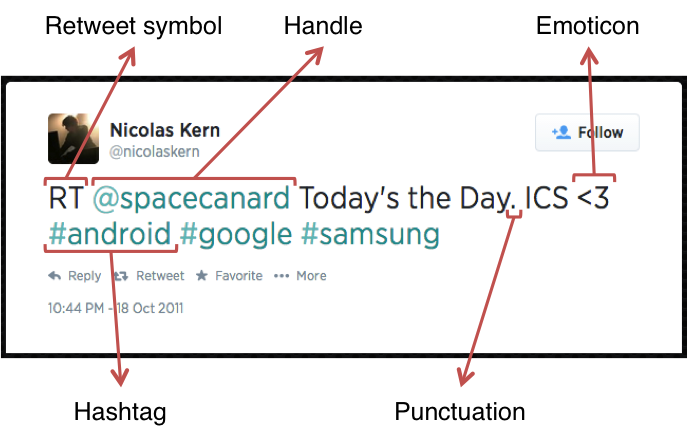
\includegraphics[width=0.75\textwidth]{img/tweet.png}
\caption{Illustration of a Tweet with various features}
\label{fig:tweet}
\end{figure}

\begin{table}[h!]
\centering

\begin{tabular}{|l|rr|rr|rr|}
\hline
 & \multicolumn{2}{c|}{Twitter Sentiment}
 & \multicolumn{2}{c|}{Stanford Corpus}
 & \multicolumn{2}{c|}{Both} \\\hline
Features	& \multicolumn{1}{c}{Avg.} & \multicolumn{1}{c|}{Max.}
			& \multicolumn{1}{c}{Avg.} & \multicolumn{1}{c|}{Max.}
			& \multicolumn{1}{c}{Avg.} & \multicolumn{1}{c|}{Max.} \\\hline
Handles		&  0.6761 &  8 &  0.4888 & 10 &  0.5804 & 10 \\
Hashtags	&  2.0276 & 13 &  0.0282 & 11 &  1.0056 & 13 \\
Urls		&  0.4431 &  4 &  0.0452 &  2 &  0.2397 &  4 \\
Emoticons	&  0.0550 &  3 &  0.0154 &  4 &  0.0348 &  4 \\
Words		& 14.4084 & 31 & 13.2056 & 33 & 13.7936 & 33 \\\hline

\end{tabular}

\caption{Frequency of Features per Tweet}
\label{tab:feat_freq}
\end{table}

\subsubsection{Hashtags} A hashtag is a word or an un-spaced phrase prefixed
with the hash symbol (\#). These are used to both naming subjects and phrases
that are currently in trending topics. For example, {\#}iPad, {\#}news

Regular Expression: \verb'#(\w+)'

Replace Expression: \verb'HASH_\1'

\subsubsection{Handles} Every Twitter user has a unique username. Any thing
directed towards that user can be indicated be writing their username preceded
by ‘@’. Thus, these are like proper nouns. For example, @Apple

Regular Expression: \verb'@(\w+)'

Replace Expression: \verb'HNDL_\1'

\subsubsection{URLs} Users often share hyperlinks in their tweets. Twitter
shortens them using its in-house URL shortening service, like
http://t.co/FCWXoUd8 -- such links also enables Twitter to alert users if the
link leads out of its domain. From the point of view of text classification, a
particular URL is not important. However, presence of a URL can be an important
feature. Regular expression for detecting a URL is fairly complex because of
different types of URLs that can be there, but because of Twitter’s shortening
service, we can use a relatively simple regular expression.

Regular Expression: \verb'(http|https|ftp)://[a-zA-Z0-9\./]+'

Replace Expression: \verb'URL'

\subsubsection{Emoticons} Use of emoticons is very prevalent throughout the web,
more so on micro-blogging sites. We identify the following emoticons and replace
them with a single word. \tabref{tab:emot} lists the emoticons we are currently
detecting. All other emoticons would be ignored.

\begin{table}[h!]
\centering
	\begin{tabular}{|l|llllll|}
	
	\hline
		\multicolumn{1}{|c|}{Emoticons} &
		\multicolumn{6}{c|}{Examples} \\
	\hline
	\verb+EMOT_SMILEY+ 	& \verb+:-)+ 	& \verb+:)+ 	& \verb+(:+ 	& \verb+(-:+ 	& \verb++ 	& \verb++ \\
	\verb+EMOT_LAUGH+ 	& \verb+:-D+ 	& \verb+:D+ 	& \verb+X-D+ 	& \verb+XD+ 	& \verb+xD+ 	& \verb++ \\
	\verb+EMOT_LOVE+ 	& \verb+<3+ 	& \verb+:*+ 	& \verb++ 	& \verb++ 	& \verb++ 	& \verb++ \\
	\verb+EMOT_WINK+ 	& \verb+;-)+ 	& \verb+;)+ 	& \verb+;-D+ 	& \verb+;D+ 	& \verb+(;+ 	& \verb+(-;+ \\
	\verb+EMOT_FROWN+ 	& \verb+:-(+ 	& \verb+:(+ 	& \verb+(:+ 	& \verb+(-:+ 	& \verb++ 	& \verb++ \\
	\verb+EMOT_CRY+ 	& \verb+:,(+ 	& \verb+:'(+ 	& \verb+:"(+ 	& \verb+:((+ 	& \verb++ 	& \verb++ \\
	\hline
	
	\end{tabular}
\caption{List of Emoticons}
\label{tab:emot}
\end{table}

\subsubsection{Punctuations} Although not all Punctuations are important from
the point of view of classification but some of these, like question mark,
exclamation mark can also provide information about the sentiments of the text.
We replace every word boundary by a list of relevant punctuations present at
that point. \tabref{tab:punc} lists the punctuations currently identified. We also
remove any single quotes that might exist in the text.

\begin{table}[h!]
\centering
	\begin{tabular}{|l|ll|}
	
	\hline
		\multicolumn{1}{|c|}{Punctuations} &
		\multicolumn{2}{c|}{Examples} \\
	\hline
	\verb+PUNC_DOT+ & \verb+.+ & \verb++ \\
	\verb+PUNC_EXCL+ & \verb+!+ & \verb+¡+ \\
	\verb+PUNC_QUES+ & \verb+?+ & \verb+¿+ \\
	\verb+PUNC_ELLP+ & \verb+...+ & \verb+…+ \\
	\hline

	\end{tabular}
\caption{List of Punctuations}
\label{tab:punc}
\end{table}

\subsubsection{Repeating Characters} People often use repeating characters while
using colloquial language, like ``I’m in a hurrryyyyy'', ``We won, yaaayyyyy!''
As our final pre-processing step, we replace characters repeating more than twice
as two characters.

Regular Expression: \verb'(.)\1{1,}'

Replace Expression: \verb'\1\1'

\subsubsection*{Reduction in feature space} It’s important to note that by
applying these pre-processing steps, we are reducing our feature set otherwise
it can be too sparse. \tabref{tab:reduction} lists the decrease in feature set
due to processing each of these features.

\begin{table}[h!]
\centering

\begin{tabular}{|l|rr|rr|rr|}
\hline
 & \multicolumn{2}{c|}{Twitter Sentiment}
 & \multicolumn{2}{c|}{Stanford Corpus}
 & \multicolumn{2}{c|}{Both} \\\hline
Preprocessing
			& \multicolumn{1}{c}{Words} & \multicolumn{1}{c|}{Percentage}
			& \multicolumn{1}{c}{Words} & \multicolumn{1}{c|}{Percentage}
			& \multicolumn{1}{c}{Words} & \multicolumn{1}{c|}{Percentage} \\\hline
None			& 19128 &         & 15910 &         & 31832 &         \\
Hashtags		& 18649 & 97.50\% & 15550 & 97.74\% & 31223 & 98.09\% \\
Handles			& 17118 & 89.49\% & 13245 & 83.25\% & 27383 & 86.02\% \\
Urls			& 16723 & 87.43\% & 15335 & 96.39\% & 29083 & 91.36\% \\
Emoticons		& 18631 & 97.40\% & 15541 & 97.68\% & 31197 & 98.01\% \\
Punctuations	& 13724 & 71.75\% & 11225 & 70.55\% & 22095 & 69.41\% \\
Repeatings		& 18540 & 96.93\% & 15276 & 96.02\% & 30818 & 96.81\% \\\hline
All				& 11108 & 58.07\% &  8646 & 54.34\% & 16981 & 53.35\% \\
\hline
\end{tabular}

\caption{Number of words before and after pre-processing}
\label{tab:reduction}
\end{table}
